\documentclass[a4j]{jarticle}

\usepackage[dvipdfmx]{graphicx}
\usepackage{url}
\usepackage{here}
%\usepackage{listings}
\usepackage{amsmath,amssymb}
\usepackage[dvipdfmx]{color}

\setlength{\headsep}{-5mm}
\setlength{\oddsidemargin}{0mm}
\setlength{\textwidth}{165mm}
\setlength{\textheight}{230mm}
\setlength{\footskip}{20mm}

\title{
\vspace{30mm}
{\bf 子育て支援システム}
\\
\vspace{5mm}
{\bf 内部設計書v1\\
}
\vspace{120mm}
}

\author{
\vspace{5mm}
チーム名 007\\
\vspace{5mm}
}


\begin{document}
\maketitle
\tableofcontents
\newpage

\section{モジュール設計書}
本システムのモジュール構成をフロー図として図\ref{functionselection}、図\ref{initialsetting}に示します。モジュール構成において各図形が何を意味するか図\ref{sample}に示してあります。


\begin{figure}[H]
    \begin{center}
    \resizebox{8cm}{!}{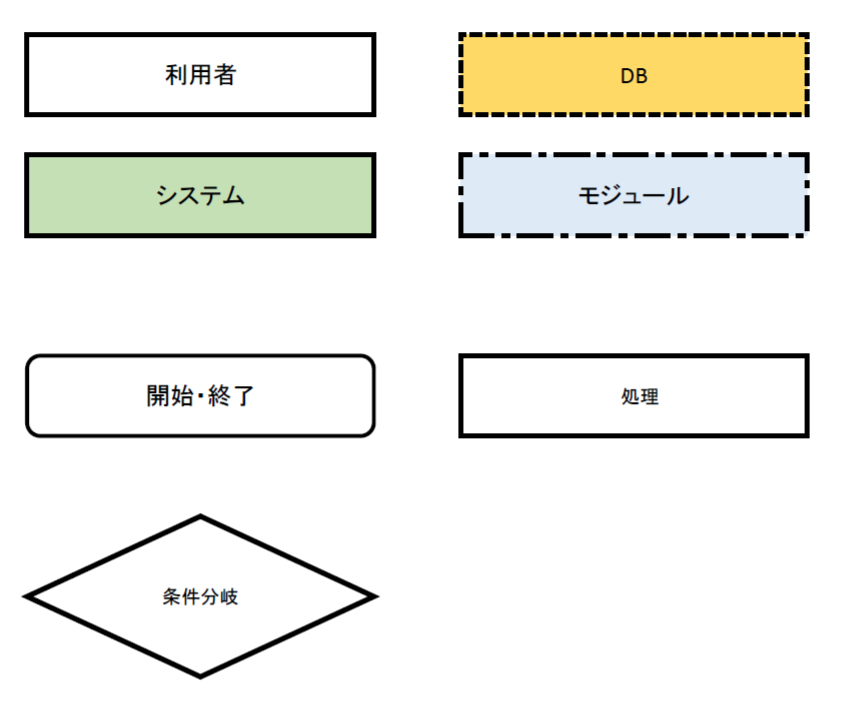
\includegraphics {sample.png}}
    \caption {見本のイメージ}
    \label{sample}
    \end{center}
\end{figure}

図\ref{sample}より、無色の図が「利用者側の操作」、緑色の図が「システム側の動作」、点線かつ黄色の図が「データベース側の動作」、点線かつ水色の図が「モジュール」を意味します。角の丸い四角形は「各モジュールの開始時・終了時の処理」、四角形は「各モジュールの処理内容」、ひし形は「条件分岐」を意味します。図及び文章中の【】はボタンを示しています。

\subsection{機能選択と初期設定}
\subsubsection{機能選択モジュール\label{機能選択}}
\begin{figure}[H]
    \begin{center}
    \resizebox{16.5cm}{!}{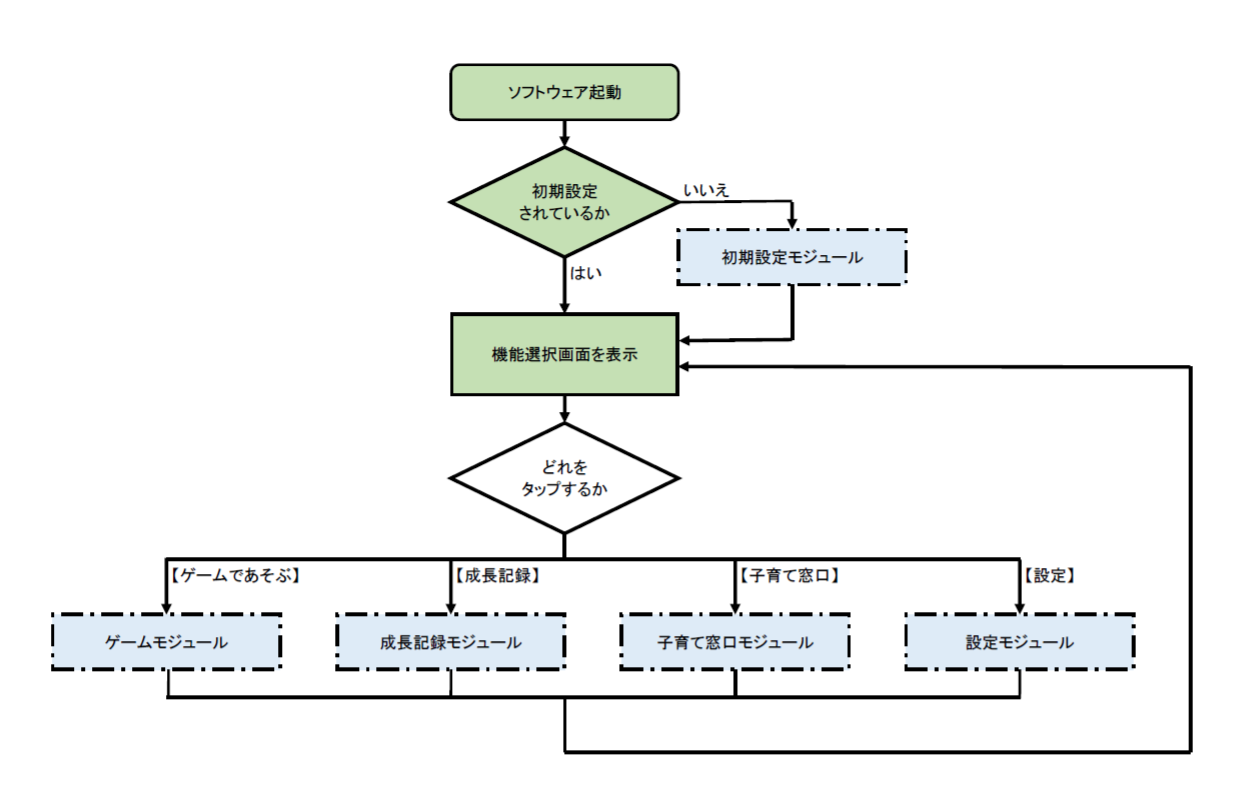
\includegraphics {functionselection.png}}
    \caption {機能選択モジュールのイメージ}
    \label{functionselection}
    \end{center}
\end{figure}

\subsubsection*{概要}
本システムを起動してから各機能選択を行う本システムのメイン画面です。

\subsubsection*{処理フロー}
\begin{itemize}
\item 本システムを起動した際に、初期設定が行われていればそのまま機能選択画面を表示させます。初期設定が行われていない場合は初期設定モジュール(第\ref{初期設定}節)を呼び出します。

\item 【ゲームであそぶ】タップすることでゲームモジュールを呼び出します。

\item 【成長記録】をタップすることで成長記録モジュール第\ref{growall}節を呼び出します。

\item 【子育て窓口】をタップすることで子育て窓口モジュールを呼び出しします。

\item 【設定】をタップすることで設定モジュールを呼び出しします。

\item 機能選択画面から呼び出される各モジュールにおいて【もどるボタン】をタップすることで、機能選択画面に戻ります。
\end{itemize}

\begin{figure}[H]
\subsubsection{初期設定モジュール\label{初期設定}}
    \begin{center}
    \resizebox{16.5cm}{!}{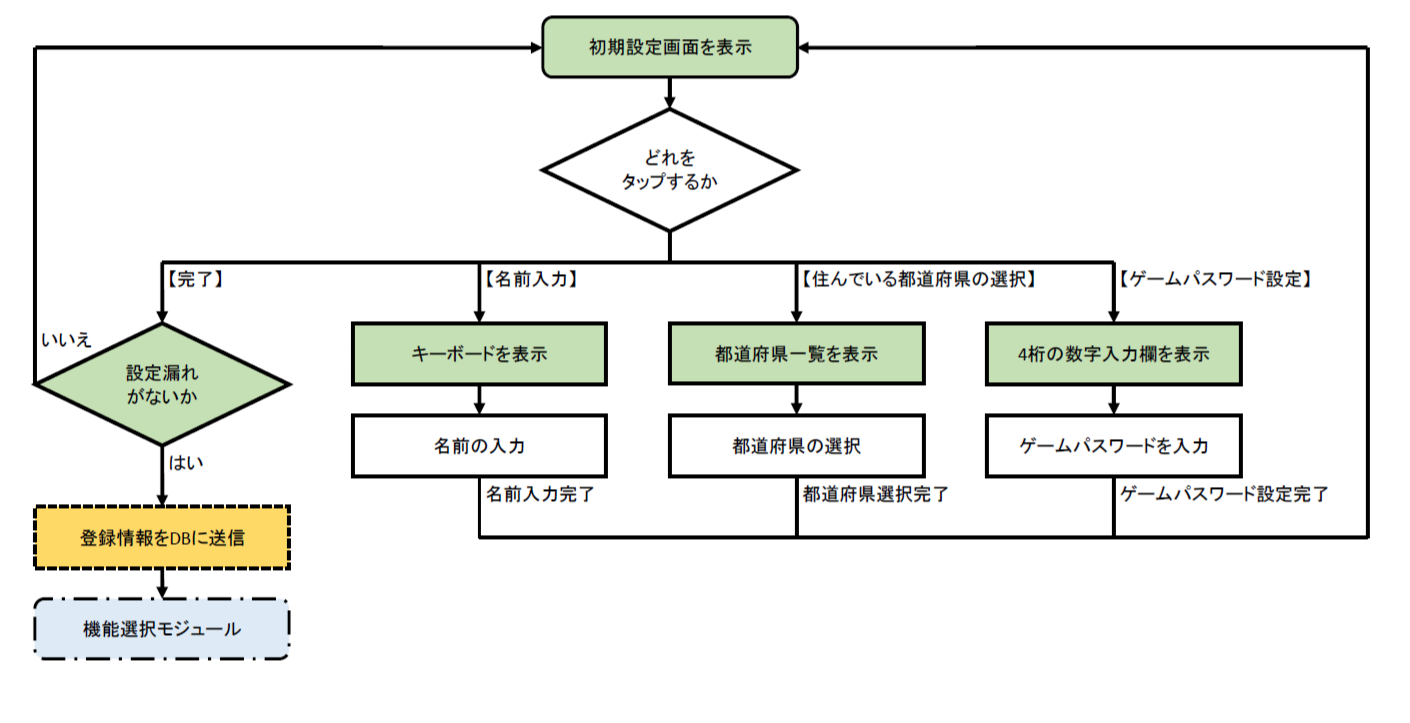
\includegraphics {initialsetting.png}}
    \caption {初期設定モジュールのイメージ}
    \label{initialsetting}
    \end{center}
\end{figure}


\subsubsection*{概要}
本システムを初めて利用する場合、最初に行う初期設定機能です。


\subsubsection*{処理フロー}
\begin{itemize}
\item 【名前(ニックネーム)の入力欄】をタップすることで画面下にキーボードが表示され、名前入力を行えるようになります。

\item 【居住地域の選択欄の矩形領域】をタップすることで47都道府県をタップして選択できるドロップダウンリストを表示させ、住んでいる地域設定が行えるようになります。

\item 【ゲームのパスワードの入力欄】をタップすることでキーボードを表示させ、ゲーム画面から機能選択画面に戻るためのパスワードとして、4桁の数字が入力できるようになります。

\item 【完了】をタップすることで初期設定が全て行われているか判定を行い、設定漏れがなければデータベースに初期設定情報を登録して機能選択画面に遷移します。設定漏れが見つかれば再び初期設定画面に戻り、設定漏れを埋めることになります。
\end{itemize}


\subsection{成長記録機能}
\subsubsection{成長記録モジュール\label{grow}}
\begin{figure}[H]
    \begin{center}
    \resizebox{16.5cm}{!}{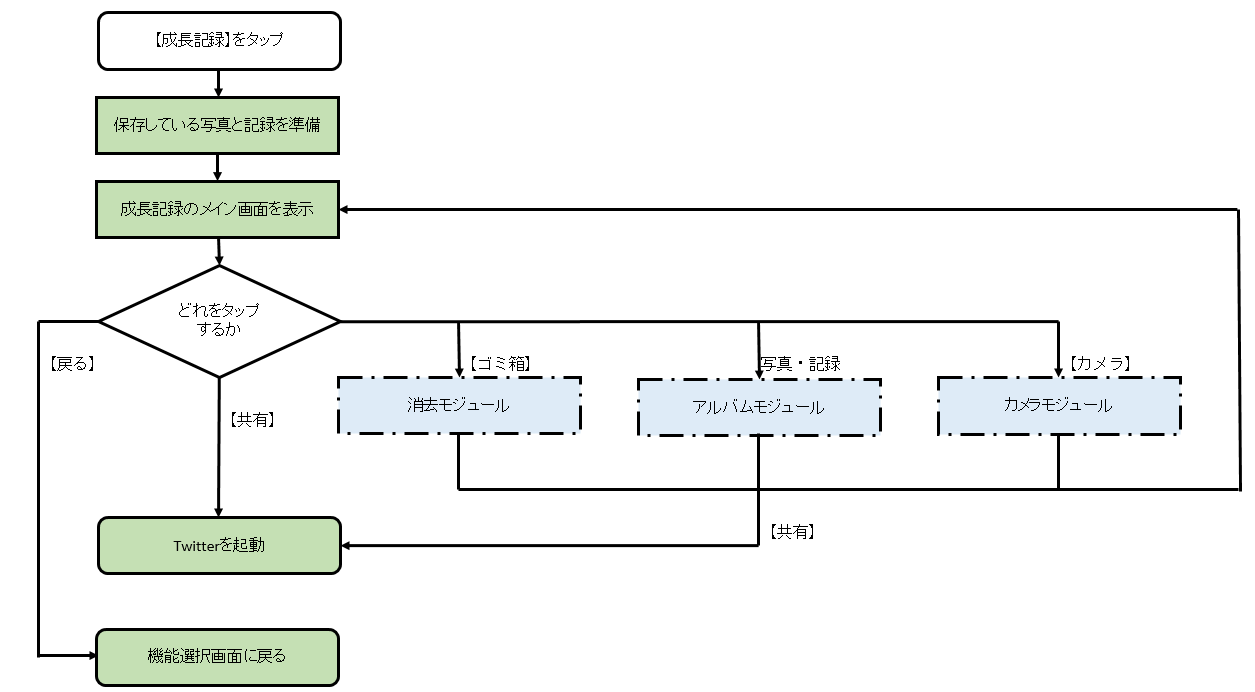
\includegraphics {growall.png}}
    \caption {成長記録モジュールのイメージ}
    \label{functionselection}
    \end{center}
\end{figure}


\subsubsection*{概要}
利用者が保存した写真やゲームの記録などの閲覧や編集などを行うために使用する成長記録のメイン画面です。

機能としては、不要な写真や記録の削除、写真や記録の閲覧、写真の撮影が行います。また、写真や記録をTwitterで共有できます。

\subsubsection*{処理フロー}
\begin{itemize}
\item 【ゴミ箱】をタップすることで削除モジュール(第\ref{delete}節)を呼び出します。

\item 写真・記録を直接タップすることでアルバムモジュール(第\ref{albam}節)を呼び出します。

\item 【カメラ】をタップすることでカメラモジュール(第\ref{camera}節)を呼び出します。

\item 【共有】をタップすることで外部アプリであるTwitterを起動します。

\item 【もどる】をタップすることで機能選択画面に戻ります。
\end{itemize}

\subsubsection{削除モジュール\label{delete}}
\begin{figure}[H]
    \begin{center}
    \resizebox{12cm}{!}{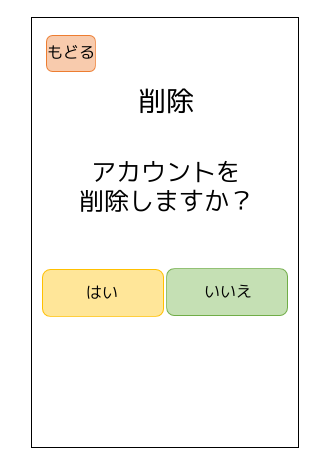
\includegraphics {delete.png}}
    \caption {削除モジュールのイメージ}
    \label{functionselection}
    \end{center}
\end{figure}

\subsubsection*{概要}
利用者が不要と判断した写真やゲームの記録の消去を行うために使用する機能です。

\subsubsection*{処理フロー}
\begin{itemize}
\item 削除したい写真や記録をタップすることでその写真や記録にチェックマークが表示されます。その後、【削除】するか【もどるボタン】を選択します。
\item 【削除】を選んだ場合確認画面が表示されます。確認画面では【はい】と【いいえ】のボタンがあります。
\item 【はい】をタップすると選択した写真や記録が削除されます。
\item 【いいえ】をタップすると削除するか戻るかを選択する画面に戻ります。
\item 【もどるボタン】をタップした場合成長記録のメイン画面に戻ります。
\end{itemize}

\subsubsection{アルバムモジュール\label{albam}}
\begin{figure}[H]
    \begin{center}
    \resizebox{16.5cm}{!}{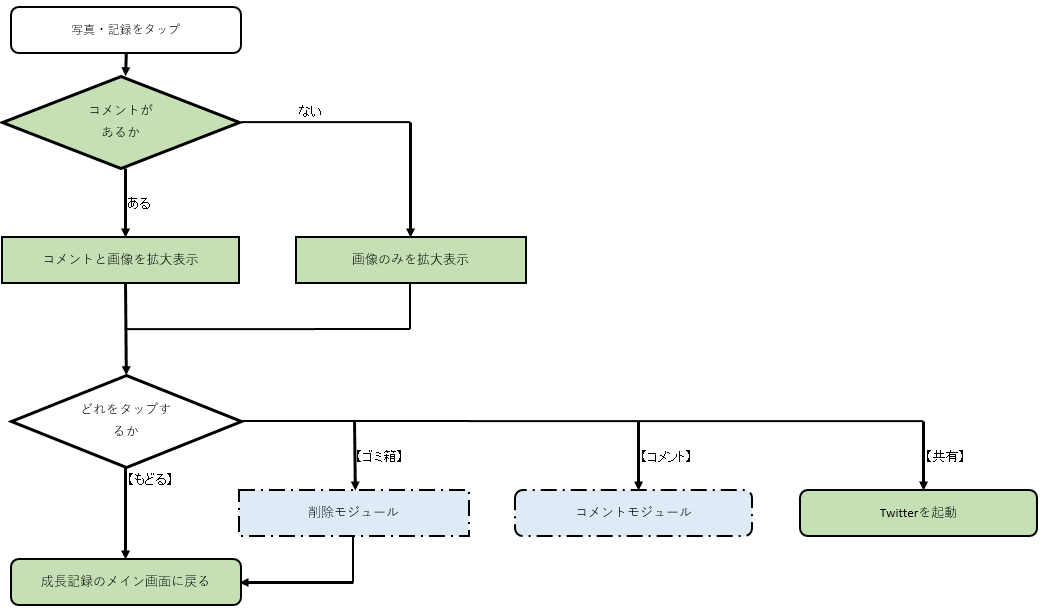
\includegraphics {albam.png}}
    \caption {アルバムモジュールのイメージ}
    \label{functionselection}
    \end{center}
\end{figure}

\subsubsection*{概要}
利用者が閲覧したい写真や記録をタップすることでそれを拡大表示して閲覧することができる機能です。

\subsubsection*{処理フロー}
\begin{itemize}
\item 写真や記録タップした場合、それにコメントがついているかを判定します。コメントがあった場合はコメントを写真や記録と一緒に表示し、ない場合は写真や記録のみを拡大表示します。拡大表示した画面では【もどる】,【ゴミ箱】,【コメント】,【共有】が選択できます。
\item 【もどる】をタップすることで成長記録のメイン画面に戻ることができます。
\item 【ゴミ箱】をタップすることで削除モジュール(第\ref{delete}節)を呼び出します。
\item 【コメント】をタップすることでコメントモジュール(第\ref{coment}節)を呼び出します。
\item 【共有】をタップすることで外部アプリであるTwitterを起動します。
\end{itemize}

\subsubsection{カメラモジュール\label{camera}}
\begin{figure}[H]
    \begin{center}
    \resizebox{8cm}{!}{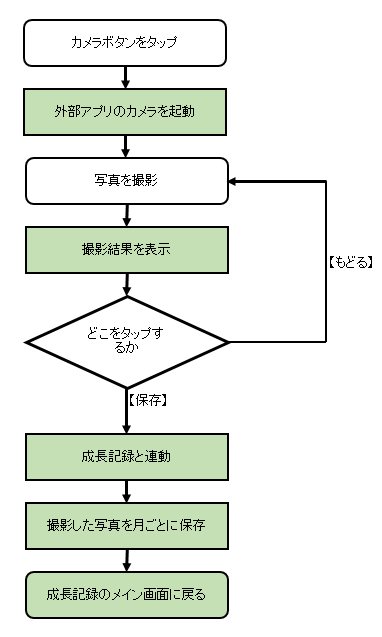
\includegraphics {camera.png}}
    \caption {カメラモジュールのイメージ}
    \label{functionselection}
    \end{center}
\end{figure}

\subsubsection*{概要}
利用者が新しく写真を撮影したいときに使用する機能です。

\subsubsection*{処理フロー}
\begin{itemize}
\item 外部アプリのカメラを起動し写真を撮影します。その後、【もどる】か【保存】を選択します。
\item 【もどるボタン】をタップすることで写真を撮影する画面に戻ります。
\item 【保存ボタン】をタップすることで成長記録と連動します。その後、撮影した写真を月ごとに保存し成長記録のメイン画面に戻ります。
\end{itemize}

\subsubsection{コメントモジュール\label{coment}}
\begin{figure}[H]
    \begin{center}
    \resizebox{16.5cm}{!}{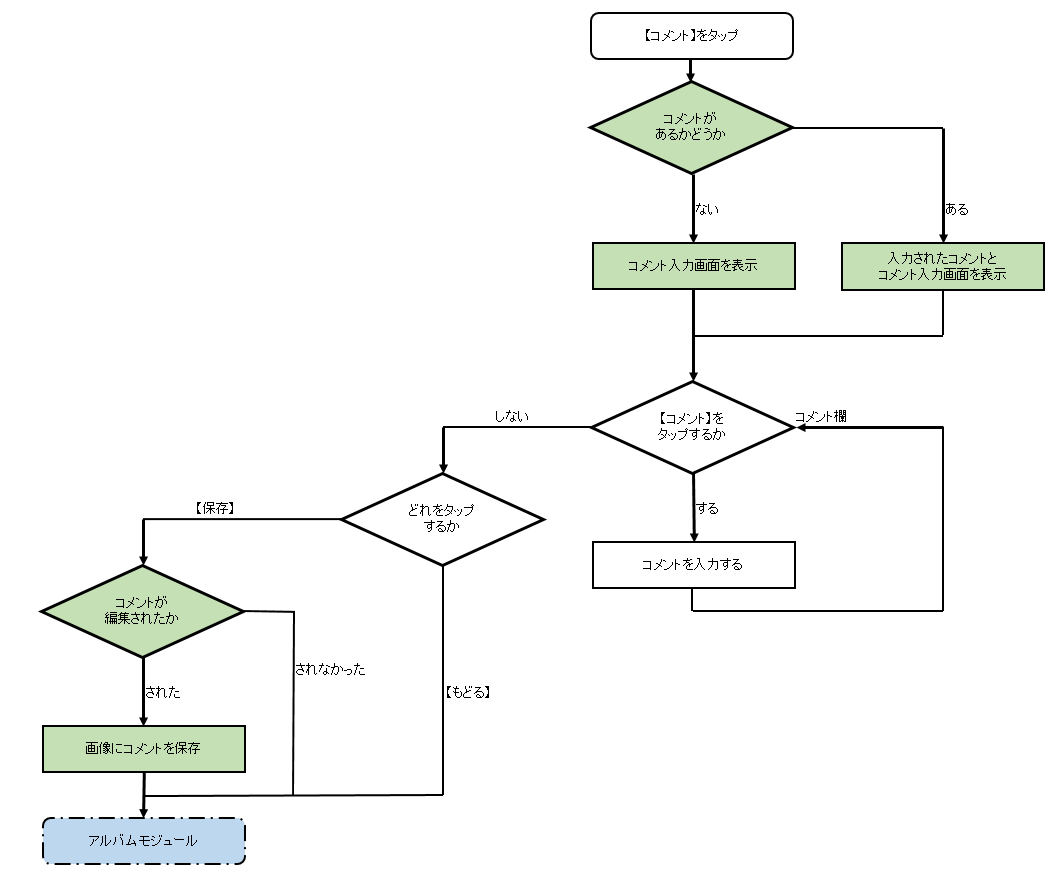
\includegraphics {coment.png}}
    \caption {コメントモジュールのイメージ}
    \label{functionselection}
    \end{center}
\end{figure}

\subsubsection*{概要}
利用者が写真や記録にコメントを挿入したい、または既についているコメントを編集したい場合に使用する機能です。

\subsubsection*{処理フロー}
\begin{itemize}
\item このモジュールに入ったときにその写真や記録にコメントが付与されているかを判定します。コメントがなければコメント入力画面のみ表示し、コメントがあればそのコメントとコメント入力画面を一緒に表示します。
\item コメント入力画面が表示されるとコメント欄をタップすることでコメントの書き込みが行えます。挿入、編集は何度でも行えます。
\item コメントの書き込みが終わった場合、もしくはコメントを書き込まなかった場合【保存】をタップするか、保存せずに【もどるボタン】をタップするかを選択します。
\item 【保存】をタップした場合コメントの内容が変更されたかを判定し、変更されていれば内容を保存してアルバムモジュールに戻ります。変更されていなければ保存せずにアルバムモジュール(第\ref{albam}節)に戻ります。
\item 【もどる】をタップすることで内容を保存せずアルバムモジュール(第\ref{albam}節)に戻ります。
\end{itemize}
\newpage


\subsection{子育て窓口機能}
\subsubsection{子育て窓口モジュール\label{子育て窓口}} %ラベル名は「~モジュール」の「~」部分を使用。他の人が参照してくる場合もあるので(メイン画面は特に)
\begin{figure}[H]
    \begin{center}
      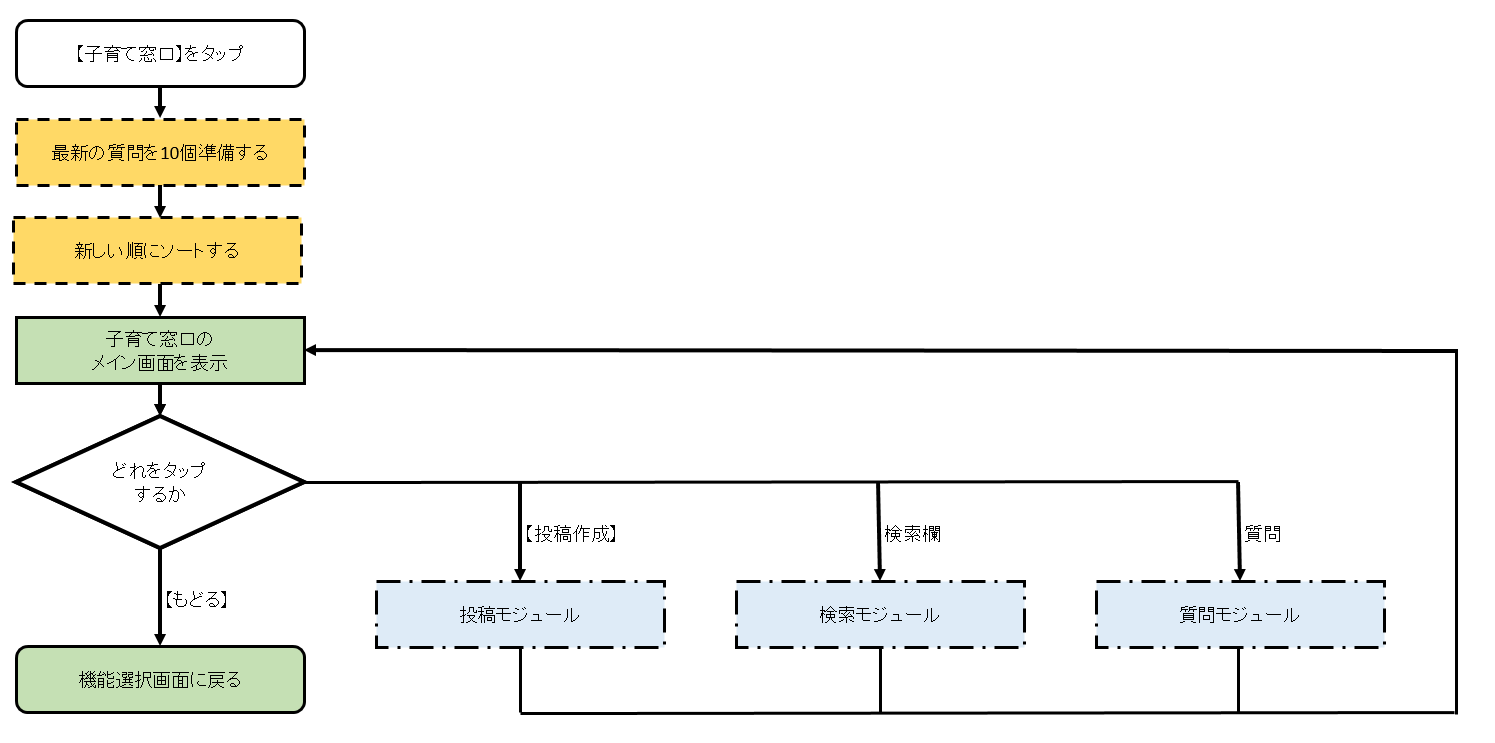
\includegraphics[height=8.0cm] {子育て窓口_全体.png} %画像は各自で用意、大きさも自分で調整
    \caption {子育て窓口モジュールのイメージ}
    \label{functionselection}
    \end{center}
\end{figure}
\subsubsection*{概要}
子育て窓口機能のメインモジュールです。子育て窓口機能の各サブシステムを利用するまでの流れを示しています。
\subsubsection*{処理フロー}
\begin{itemize}
\item データベースに保存されている最新の質問10個を要求し、新しい順に画面に表示させます。
\item 【もどる】をタップすることで機能選択画面に戻ります。
\item 【投稿作成】をタップすることで投稿モジュール(第\ref{投稿}節)を呼び出します。
\item 【検索】をタップすることで検索モジュール(第\ref{検索}節)を呼び出します。
\item 各質問をタップすることで質問モジュール(第\ref{質問}節)を呼び出します。

\end{itemize}

\subsubsection{投稿モジュール\label{投稿}} %ラベル名は「~モジュール」の「~」部分を使用。他の人が参照してくる場合もあるので(メイン画面は特に)
\begin{figure}[H]
    \begin{center}
      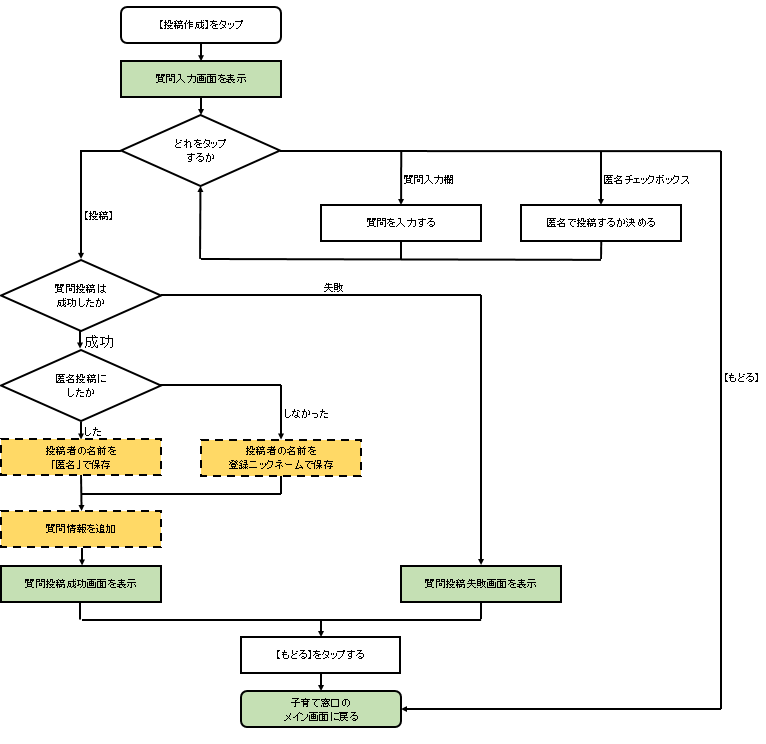
\includegraphics[height = 12.0cm] {子育て窓口_投稿.png} %画像は各自で用意、大きさも自分で調整
    \caption {投稿モジュールのイメージ}
    \label{functionselection}
    \end{center}
\end{figure}
\subsubsection*{概要}
本システム利用者が子育てに関する質問を投稿するためのモジュールです。
\subsubsection*{処理フロー}
\begin{itemize}
\item 質問入力欄をタップすることで質問を入力することができます。匿名で投稿するか、登録されているユーザ名で投稿するか決めることができ、匿名投稿をしたい場合は匿名チェックボックスをタップします。
\item 【投稿】をタップすることで投稿を行うことができます。
\item 投稿に失敗した場合は質問投稿失敗画面を表示させます。
\item 投稿に成功した場合はユーザ名と質問情報をデータベースに保存します。匿名チェックボックスをタップしていた場合は、ユーザ名を「匿名」で保存します。
\item 投稿に成功した場合は質問投稿成功画面を表示させます。
\item 投稿終了後、【もどる】をタップすることで子育て窓口機能のメイン画面に戻ります。

\end{itemize}

\subsubsection{検索モジュール\label{検索}} %ラベル名は「~モジュール」の「~」部分を使用。他の人が参照してくる場合もあるので(メイン画面は特に)
\begin{figure}[H]
    \begin{center}
      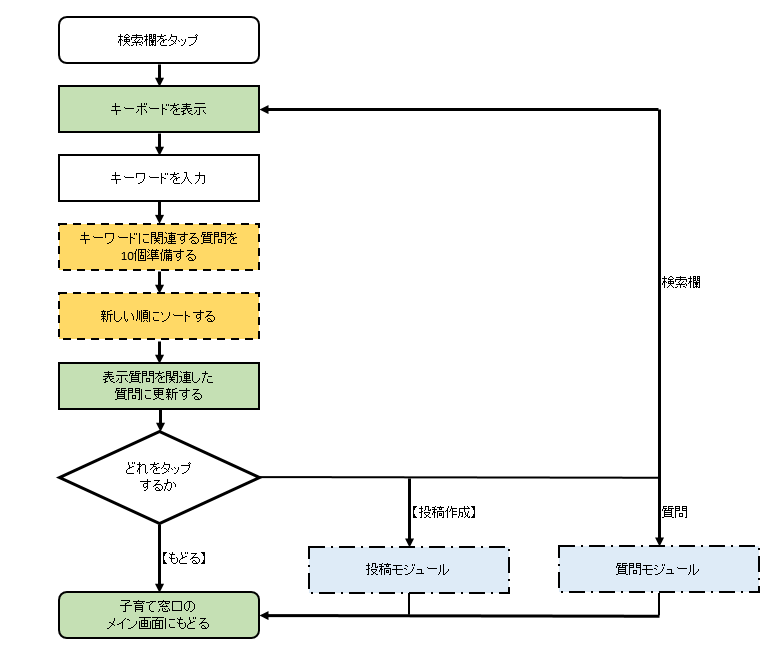
\includegraphics[height = 12.0cm] {子育て窓口_検索.png} %画像は各自で用意、大きさも自分で調整
    \caption {検索モジュールのイメージ}
    \label{functionselection}
    \end{center}
\end{figure}
\subsubsection*{概要}
本システム利用者が子育てに関する質問をキーワードで検索し、キーワードに関連した質問を表示させるためのモジュールです。
\subsubsection*{処理フロー}
\begin{itemize}
\item 検索欄をタップすることでキーボードが表示され、キーワードを入力することができます。入力されたキーワードに関連する質問10個をデータベースに要求し、新しい順に画面に表示させます。
\item 【もどる】をタップすることで子育て窓口機能のメイン画面に戻ります。
\item 【投稿作成】をタップすることで投稿モジュール(第\ref{投稿}節)を呼び出します。
\item 各質問をタップすることで質問モジュール(第\ref{質問}節)を呼び出します。


\end{itemize}

\subsubsection{質問モジュール\label{質問}} %ラベル名は「~モジュール」の「~」部分を使用。他の人が参照してくる場合もあるので(メイン画面は特に)
\begin{figure}[H]
    \begin{center}
      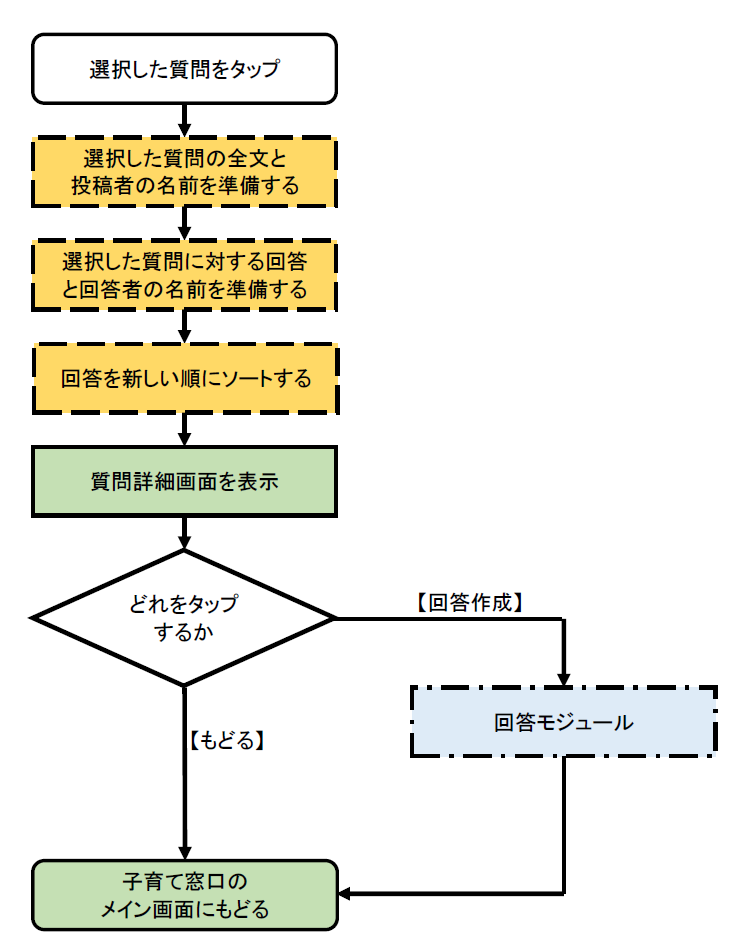
\includegraphics[height = 12.0cm] {子育て窓口_質問.png} %画像は各自で用意、大きさも自分で調整
    \caption {質問モジュールのイメージ}
    \label{functionselection}
    \end{center}
\end{figure}
\subsubsection*{概要}
画面上に表示された各質問をタップしたときに利用するモジュールです。質問の詳細内容を表示させます。
\subsubsection*{処理フロー}
\begin{itemize}
\item データベースに質問の全文と投稿者のユーザ名を要求し、画面に表示させます。
\item データベースに質問に対する回答の全文と回答者のユーザ名を要求し、画面に表示させます。
\item 【もどる】をタップすることで子育て窓口機能のメイン画面に戻ります。
\item 【回答作成】をタップすることで回答モジュール(第\ref{回答}節)を呼び出します。

\end{itemize}

\subsubsection{回答モジュール\label{回答}} %ラベル名は「~モジュール」の「~」部分を使用。他の人が参照してくる場合もあるので(メイン画面は特に)
\begin{figure}[H]
    \begin{center}
      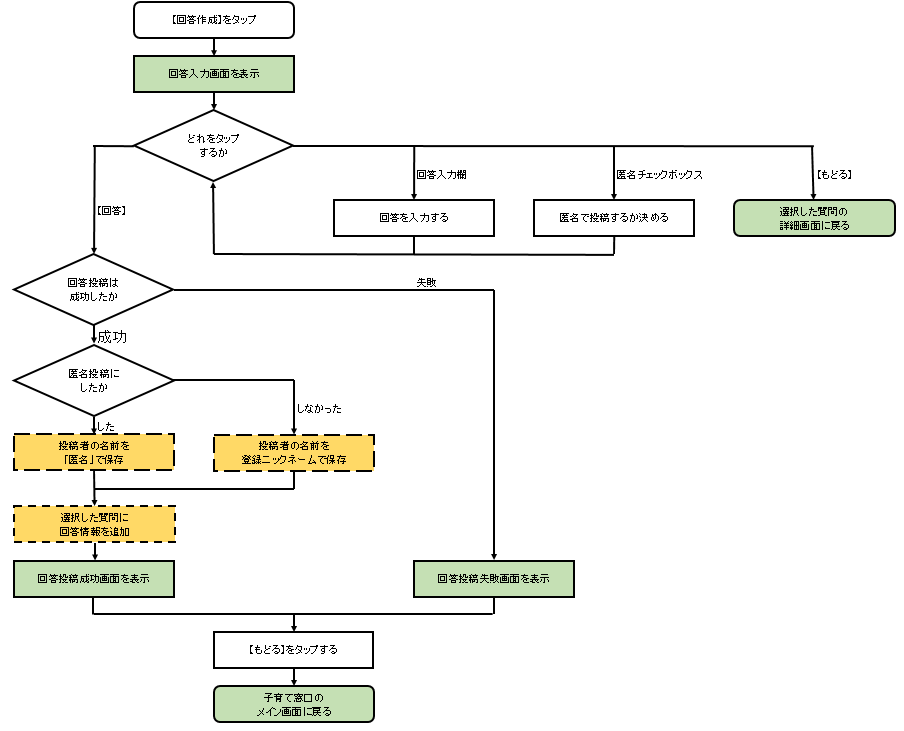
\includegraphics[height = 12.0cm] {子育て窓口_回答.png} %画像は各自で用意、大きさも自分で調整
    \caption {回答モジュールのイメージ}
    \label{functionselection}
    \end{center}
\end{figure}
\subsubsection*{概要}
子育てに関する質問に対して回答を行うためのモジュールです。
\subsubsection*{処理フロー}
\begin{itemize}
\item 回答入力欄をタップすることで回答を入力することができます。匿名で投稿するか、登録されているユーザ名で投稿するか決めることができ、匿名投稿をしたい場合は匿名チェックボックスをタップします。
\item 【回答】をタップすることで投稿を行うことができます。
\item 投稿に失敗した場合は回答投稿失敗画面を表示させます。
\item 投稿に成功した場合はユーザ名と回答情報をデータベースに保存します。匿名チェックボックスをタップしていた場合は、ユーザ名を「匿名」で保存します。
\item 投稿に成功した場合は回答投稿成功画面を表示させます。
\item 投稿終了後、【もどる】をタップすることで子育て窓口機能のメイン画面に戻ります。

\end{itemize}


\subsection{設定機能}
\subsubsection{設定機能モジュール\label{設定機能}} %ラベル名は「~モジュール」の「~」部分を使用。他の人が参照してくる場合もあるので(メイン画面は特に)
\begin{figure}[H]
    \begin{center}
      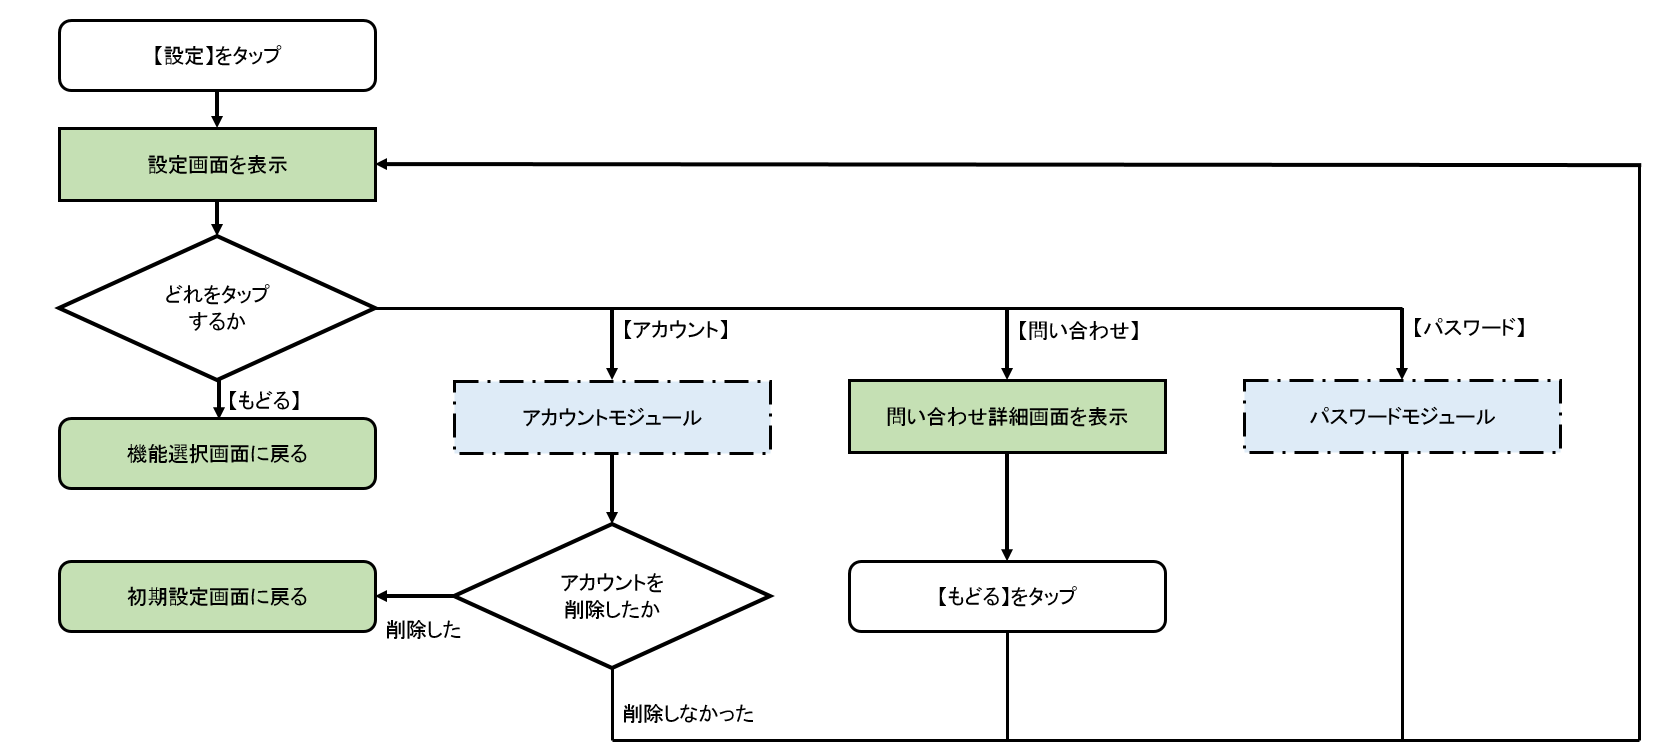
\includegraphics[height=8.0cm] {設定_全体.png} %画像は各自で用意、大きさも自分で調整
    \caption {設定機能モジュールのイメージ}
    \label{functionselection}
    \end{center}
\end{figure}
\subsubsection*{概要}
本システムはSNS機能を利用する際に必要なアカウントの登録を行うことができます。また。アカウントの変更・削除も行うことができます。他に、こどもがゲーム機能を使用する際に他の機能や本システム以外のシステムを触らないようにパスワードの設定も行います。
\subsubsection*{処理フロー}
\begin{itemize}
\item 【アカウント】をタップすることでアカウントモジュールを呼び出します。その後アカウントが削除されたかどうかで設定画面か初期設定画面に遷移します。

\item 【問い合わせ】ボタンをタップすることで問い合わせ詳細画面を表示します。その後【もどる】ボタンをタップすることで設定画面に戻ります。

\item 【パスワード】をタップすることでパスワードモジュールを呼び出します。

\item 【もどる】をタップすることで機能設定画面に戻ります。
\end{itemize}

\subsubsection{アカウントモジュール\label{アカウント}} %ラベル名は「~モジュール」の「~」部分を使用。他の人が参照してくる場合もあるので(メイン画面は特に)
\begin{figure}[H]
    \begin{center}
      \resizebox{16.5cm}{!}{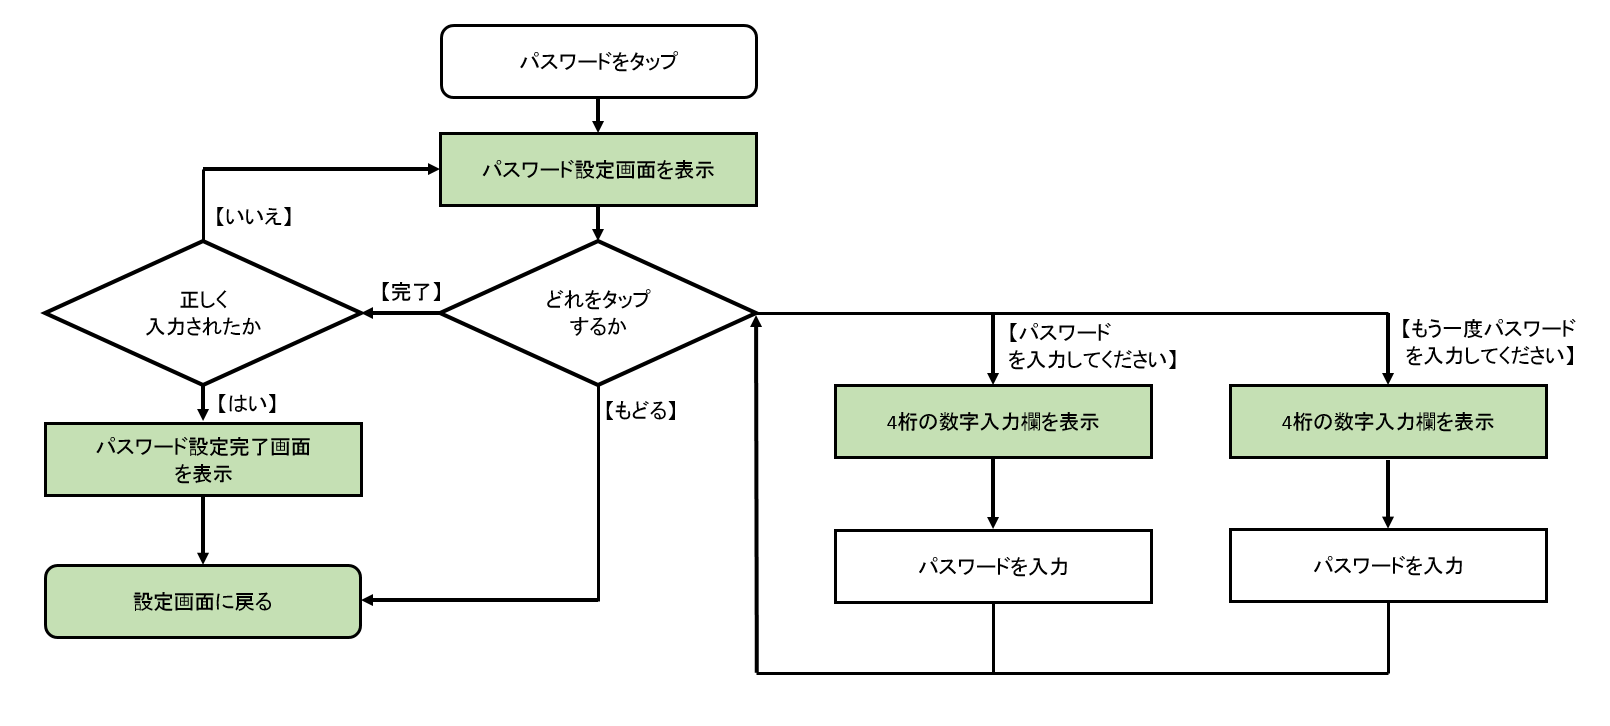
\includegraphics{設定_パスワード.png}} %画像は各自で用意、大きさも自分で調整
    \caption {アカウントモジュールのイメージ}
    \label{functionselection}
    \end{center}
\end{figure}
\subsubsection*{概要}
SNSを利用する際のアカウントの登録・変更・削除を行う機能です。
\subsubsection*{処理フロー}
\begin{itemize}
\item 【変更】をタップすることで変更モジュールを呼び出します。
\item 【削除】をタップすることで削除モジュールを呼び出します。
\item 【もどる】をタップすることで設定画面に戻ります。
\end{itemize}

\subsubsection{変更モジュール\label{変更}} %ラベル名は「~モジュール」の「~」部分を使用。他の人が参照してくる場合もあるので(メイン画面は特に)
\begin{figure}[H]
    \begin{center}
      \resizebox{16.5cm}{!}{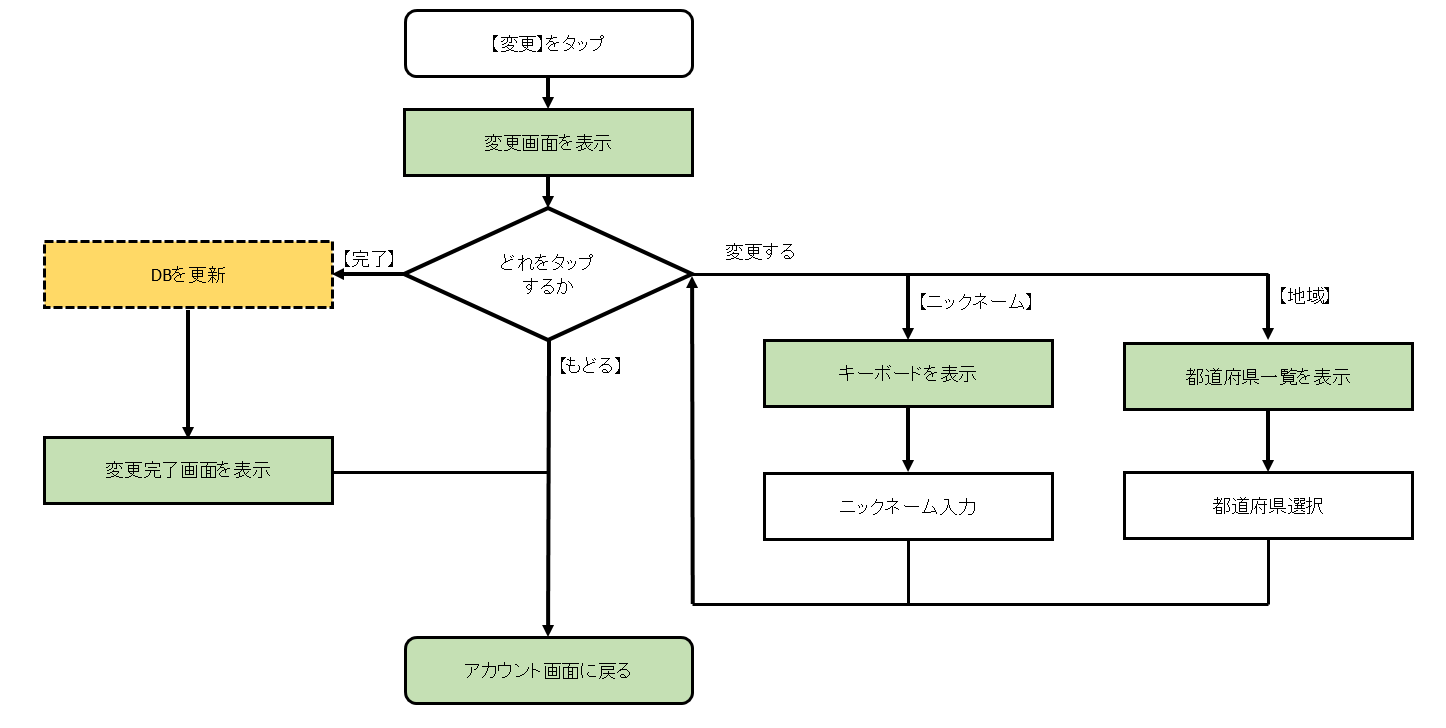
\includegraphics{設定_変更.png}}%画像は各自で用意、大きさも自分で調整
    \caption {変更モジュールのイメージ}
    \label{functionselection}
    \end{center}
\end{figure}
\subsubsection*{概要}
アカウントの変更を行う機能です。
\subsubsection*{処理フロー}
\begin{itemize}
\item 【ニックネーム】をタップすることでニックネームの変更を行います。
\item 【地域】をタップすることで地域の変更を行います。
\item 【完了】をタップした場合【ニックネーム】と【地域】の設定が正しく行われていればDBを更新しアカウントの変更を行います。
\item 【もどる】ボタンをタップすることでアカウント画面に戻ります。
\end{itemize}

\subsubsection{削除モジュール\label{削除}} %ラベル名は「~モジュール」の「~」部分を使用。他の人が参照してくる場合もあるので(メイン画面は特に)
\begin{figure}[H]
    \begin{center}
      \resizebox{16.5cm}{!}{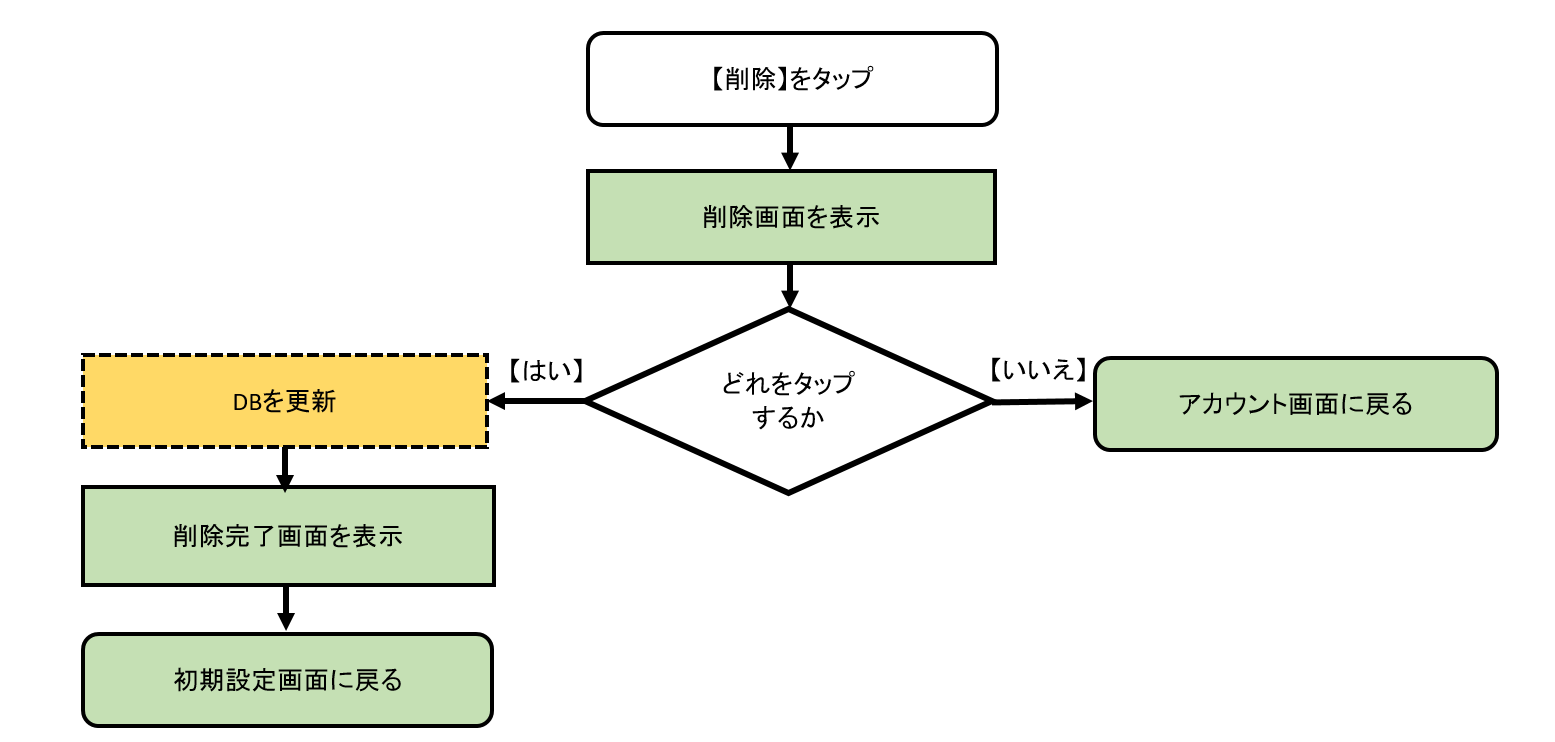
\includegraphics{設定_削除.png}} %画像は各自で用意、大きさも自分で調整
    \caption {削除モジュールのイメージ}
    \label{functionselection}
    \end{center}
\end{figure}
\subsubsection*{概要}
アカウントの削除を行うモジュールです。
\subsubsection*{処理フロー}
\begin{itemize}
\item 【はい】をタップすることでDBを更新しアカウントの削除を行います。その後削除完了画面を表示し初期設定画面に戻ります。
\item 【いいえ】をタップすることでアカウント画面に戻ります。
\end{itemize}

\subsubsection{パスワードモジュール\label{パスワード}} %ラベル名は「~モジュール」の「~」部分を使用。他の人が参照してくる場合もあるので(メイン画面は特に)
\begin{figure}[H]
    \begin{center}
       \resizebox{16.5cm}{!}{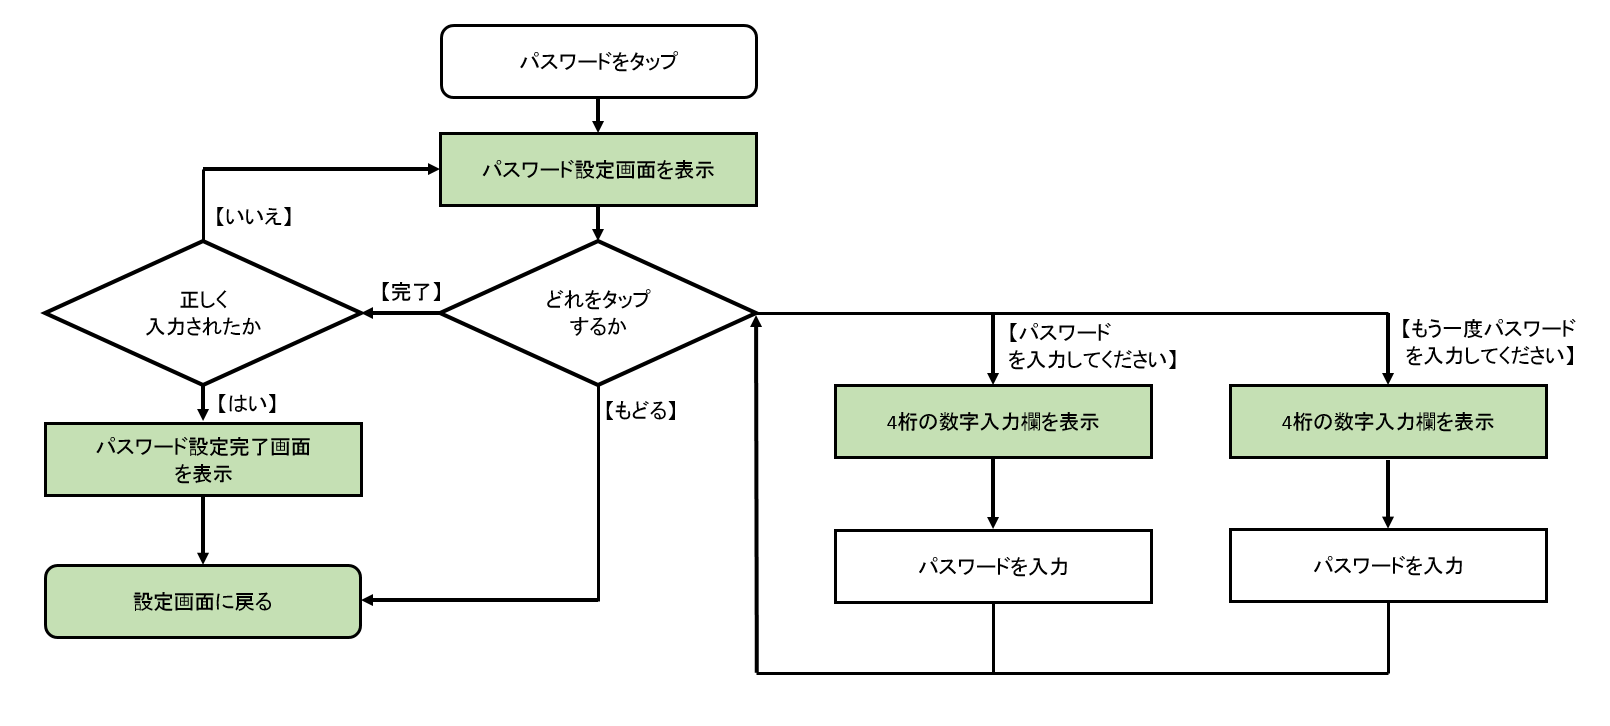
\includegraphics{設定_パスワード.png}}%画像は各自で用意、大きさも自分で調整
    \caption {パスワードモジュールのイメージ}
    \label{functionselection}
    \end{center}
\end{figure}
\subsubsection*{概要}
こどもがゲーム機能を利用する際に他の機能や他のシステムを利用できないようにパスワードを設定する機能です。
\subsubsection*{処理フロー}
\begin{itemize}
\item 【パスワードを入力してください】をタップし4桁の数字を入力することでパスワードの設定を行います。
\item【もう一度パスワードを入力してください】をタップし4桁のパスワードを入力することでパスワードの確認を行います。
\item 【完了】をタップした場合パスワードが正しく入力されていればパスワード設定画面完了画面を表示し設定画面に戻ります。正しく入力されていなければパスワード設定画面に戻ります。
\item 【もどる】をタップすることで設定画面に戻ります。
\end{itemize}

\subsection{見本機能}
\begin{figure}[H]
    \begin{center}
    \resizebox{16.5cm}{!}{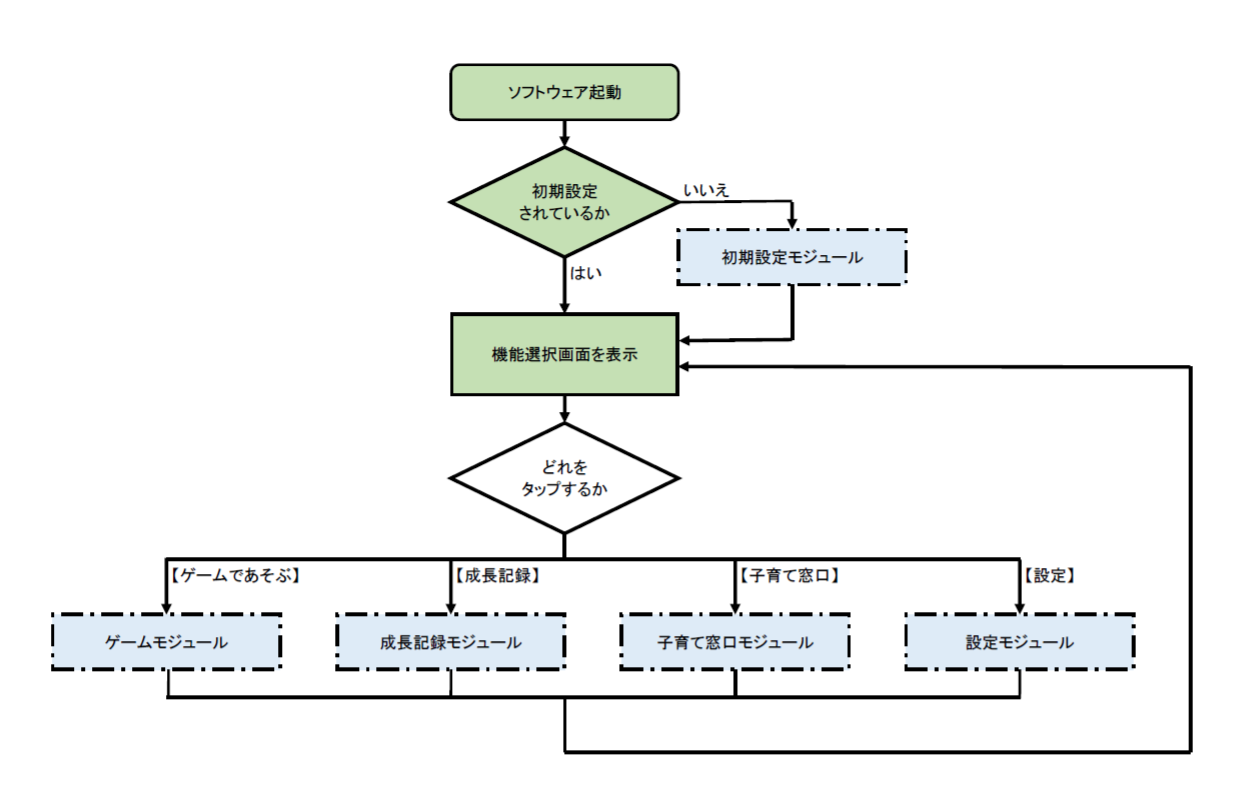
\includegraphics {functionselection.png}} %画像は各自で用意、大きさも自分で調整
    \caption {見本モジュールのイメージ}
    \label{functionselection}
    \end{center}
\end{figure}
\subsubsection{見本モジュール\label{見本}} %ラベル名は「~モジュール」の「~」部分を使用。他の人が参照してくる場合もあるので(メイン画面は特に)
\subsubsection*{概要}
モジュールの概要説明をここで行います。
\subsubsection*{処理フロー}
\begin{itemize}
\item 【A】をタップすることで~モジュール(第\ref{初期設定}節)を呼び出します。%()は半角で!
\item 【B】
\item 【C】
\item 【D】
\end{itemize}

\end{document}
